\begin{figure*}
\centering
\begin{subfigure}[b]{0.48\textwidth}
    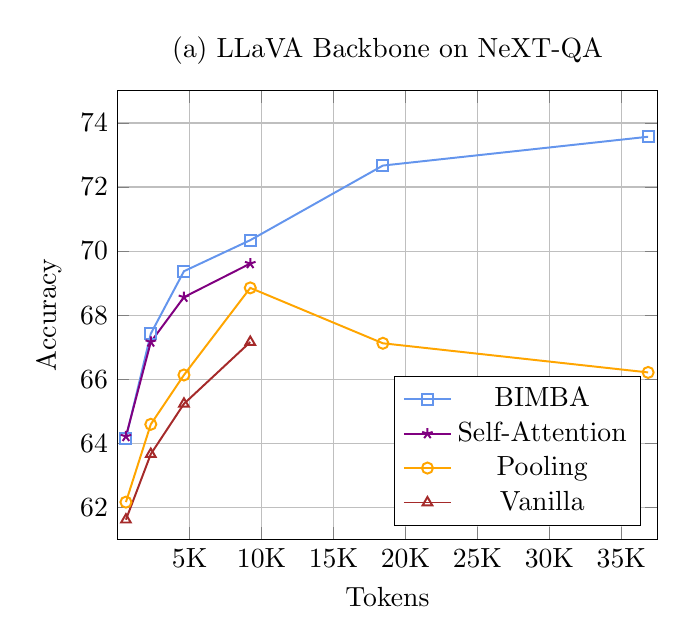
\begin{tikzpicture}
    \begin{axis}[
        % width=12cm, height=8cm,
        xlabel={Tokens},
        ylabel={Accuracy},
        title={(a) LLaVA Backbone on NeXT-QA},
        xmin=0, xmax=37500,
        ymin=61, ymax=75,
        %xtick={576, 2304, 4608, 9216, 18432, 36864},
        % xticklabels={576, 2304, 4608, 9216, 18432, 36864},
        xtick={5000, 10000, 15000, 20000,25000,30000, 35000},
        xticklabels={5K, 10K, 15K, 20K, 25K,30K, 35K},
        ytick={60, 62, 64, 66, 68, 70, 72, 74},
        legend pos=south east,
        grid=both,
        scaled ticks = false,
        scaled x ticks = false,
        % xmode=log,
        % log basis x=1
    ]
    % BIMBA Data
    \addplot[line width=.25mm, color=CornflowerBlue, mark=square, mark size=2pt]
    coordinates {
    (576, 64.16) (2304, 67.42) (4608, 69.37) (9216, 70.34) (18432, 72.67) (36864, 73.57)
    };
    \addlegendentry{BIMBA}
    
    % Self-Attention Data
    \addplot[line width=.25mm, color=Purple, mark=star, mark size=2pt]
        coordinates {
        (576, 64.21) (2304, 67.16) (4608, 68.56) (9216, 69.61)
    };
    \addlegendentry{Self-Attention}
    
    % Pooling Data
    \addplot[line width=.25mm, color=Orange, mark=o, mark size=2pt]
    coordinates {
    (576, 62.16) (2304, 64.59) (4608, 66.13) (9216, 68.85) (18432, 67.12) (36864, 66.21)
    };
    \addlegendentry{Pooling}

    \addplot[line width=.25mm, color=Brown, mark=triangle, mark size=2pt]
    coordinates {
    (576, 61.61) (2304, 63.66) (4608, 65.23) (9216, 67.16) 
    };
    \addlegendentry{Vanilla}

    \end{axis}
    \end{tikzpicture}
% \caption{Figure 1}
\end{subfigure}
\hfill
\begin{subfigure}[b]{0.48\textwidth}
    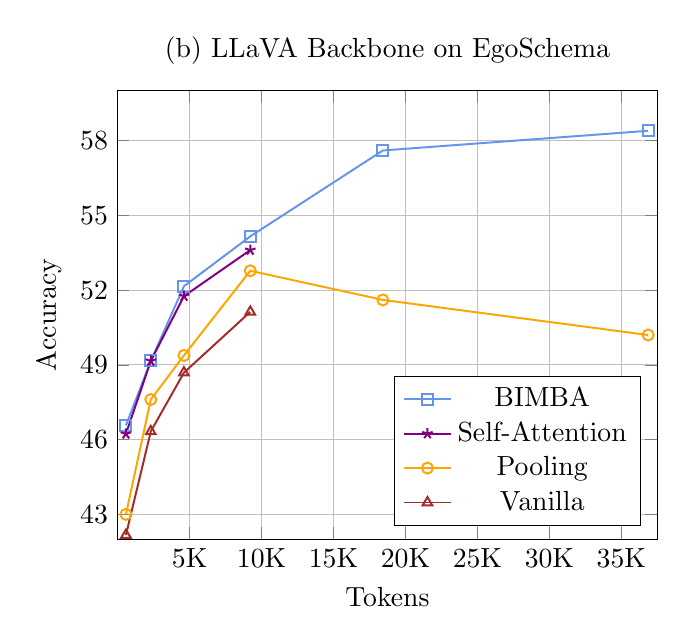
\begin{tikzpicture}
    \begin{axis}[
        % width=12cm, height=8cm,
        xlabel={Tokens},
        ylabel={Accuracy},
        title={(b) LLaVA Backbone on EgoSchema},
        xmin=0, xmax=37500,
        ymin=42, ymax=60,
        %xtick={576, 2304, 4608, 9216, 18432, 36864},
        % xticklabels={576, 2304, 4608, 9216, 18432, 36864},
        xtick={5000, 10000, 15000, 20000,25000,30000, 35000},
        xticklabels={5K, 10K, 15K, 20K, 25K,30K, 35K},
        ytick={43, 46, 49, 52, 55, 58, 61},
        legend pos=south east,
        grid=both,
        scaled ticks = false,
        scaled x ticks = false,
        % xmode=log,
        % log basis x=1
    ]
    % BIMBA Data
    \addplot[line width=.25mm, color=CornflowerBlue, mark=square, mark size=2pt]
    coordinates {
    (576, 46.57) (2304, 49.16) (4608, 52.16) (9216, 54.16) (18432, 57.61) (36864, 58.40)
    };
    \addlegendentry{BIMBA}

    % Self-Attention Data
    \addplot[line width=.25mm, color=Purple, mark=star, mark size=2pt]
        coordinates {
        (576, 46.23) (2304, 49.16) (4608, 51.76) (9216, 53.61)
    };
    \addlegendentry{Self-Attention}

    % Pooling Data
    \addplot[line width=.25mm, color=Orange, mark=o, mark size=2pt]
    coordinates {
    (576, 43.00) (2304, 47.61) (4608, 49.38) (9216, 52.78) (18432, 51.61) (36864, 50.20)
    };
    \addlegendentry{Pooling}

    \addplot[line width=.25mm, color=Brown, mark=triangle, mark size=2pt]
    coordinates {
    (576, 42.17) (2304, 46.33) (4608, 48.69) (9216, 51.13) 
    };
    \addlegendentry{Vanilla}
    
    \end{axis}
    \end{tikzpicture}
    % \caption{Figure 2}
\end{subfigure}
\caption{Performance Using LLaVA Backbone}
\label{fig:performance llava}
\end{figure*}



